\documentclass[10pt]{article}
\usepackage[utf8]{inputenc}
\usepackage[spanish]{babel}
\usepackage{amsmath}
\usepackage{epsfig}
\usepackage{enumerate}
\usepackage{float}
\usepackage{listings}
\frenchspacing
\linespread{1.2}                                          %espacio entre líneas
\setlength{\parskip}{1.5ex plus 0.2ex minus 0.2ex}        %espacio entre párrafos
\setlength{\columnsep}{0.9cm}  				  %espacio entre columnas
\usepackage{indentfirst}
\usepackage{graphicx}
\usepackage{verbatim}
\usepackage{url}
\usepackage{multicol}
\usepackage{geometry}
\usepackage{fancyhdr}
\usepackage{moreverb}
\usepackage{hyperref}

\geometry{tmargin=3.0cm, lmargin=3.0cm, rmargin=2.5cm, bmargin=3.0cm}

\newcommand\R{R}
\newenvironment{keywords}{\begin{description}\item[Palabras Claves:]}{\end{description}}
%\renewcommand{\refname}{Referencias}
%\renewcommand\listfigurename{Lista de Figuras}
%\renewcommand\listoftables{Lista de Tablas}


\title{
\center{\emph{Desarrollo de una plataforma astroinformática para la administración y análisis inteligente de datos a gran escala} \\}
\center{\textbf{Nombre del documento} \\}
\author{
        Mauricio Solar, Marcelo Mendoza, Jonathan Antognini, Walter Fariña, \\
        Jorge Ibsen, Lars Nyman,
        Eduardo Vera, Diego Mardones, Guillermo Cabrera,\\
        Paola Arellano,
        Karim Pichara, Nelson Padilla,
        Ricardo Contreras, \\ Neil Nagar,
        Victor Parada.
}
\date{Ciudad, \today}
}

\begin{document}
\maketitle

\vspace{0.5cm}

\begin{center}
	\begin{abstract}
	Abstract del documento.
	\end{abstract}
\end{center}

\vspace{0.4cm}

\begin{center}
\begin{keywords}
	Palabras claves del documento.
\end{keywords}
\end{center}

\vspace{1cm}

\thispagestyle{empty}

\newpage

\section{Resumen Ejecutivo}

\newpage

\tableofcontents
\newpage

\listoffigures
\newpage

\listoftables
\newpage

\section{Metodología de Trabajo}

En primer lugar se debe establecer que existe 2 grandes áreas de trabajo, una encargada de la investigación y otra encargada del desarrollo de la aplicación. En base a esta división, se ha establecido dos coordinadores por área, quienes son los encargados de establecer el contacto directo con los investigadores en el ámbito de la astronomía, computación y astroingeniería por un lado, y los desarrolladores por el otro. Ambos coordinadores a su vez, velan por la integración de los resultados de la investigación científica con el desarrollo tecnológico de la herramienta denominada Observatorio Virtual.

En el área de desarrollo, para esta etapa, se ha definido 3 equipos de trabajo: uno encargado de la ingestión de datos. Este equipo es encargado de tomar principalmente los datos del mandante (ALMA) y otros que puedan ser incluidos y poblar la base de datos de ChiVO; el segundo equipo trabajó en la integración y pruebas del sistema. En este contexto se terminó de integrar las 3 capas del sistema (\emph{backend}, \emph{endpoint} y \emph{frontend}) y se probó su funcionamiento en la infraestructura destinada para el sistema en producción; el tercer equipo se encargó de migrar todo el desarrollo a la infraestructura de producción, afinando algunos detalles que quedaban por corregir en el sitio web.

Cada uno de los equipos se reunía periódicamente para trabajar en las labores designadas, y semanalmente se realizaba una reunión con los 3 equipos para coordinar acciones en conjunto.

Por otro lado, una vez al mes se realizaba una reunión de coordinación con todos los actores relacionados al proyecto, donde se coordinaba aspectos técnicos, científicos y de administración del proyecto. En estas reuniones se coordinaba además, encuentros entre el coordinador de investigación con los investigadores de todas las universidades participantes, cuando fuere pertinente.

Toda la documentación se maneja en una plataforma en la nube para el almacenamiento de archivos, lo que permite una fácil y rápida colaboración entre los participantes de diferentes universidades del país integrantes del proyecto. Además, la codificación de la aplicación se maneja bajo un sistema de control de versiones distribuido, lo que permite el trabajo de los diferente equipos de desarrollo sin mayores problemas.


\newpage

\section{Definición del Problema}

El problema abordado para este hito es la puesta en marcha
del prototipo funcional de ChiVO. Esto implica integrar los
distintos subsistemas desarrollados para el observatorio
virtual Chileno en sus versiones básicas. En el Hito 1 
se detalló el proceso de captura de requerimientos, de 
los cuales se seleccionaron los siguientes para el 
desarrollo del prototipo:

\begin{enumerate}
\item Buscar por coordenadas o región del cielo:
Se podrán realizar búsquedas de posición mediante coordenadas y radio angular
(cónicas) o por región del cielo.
\item Buscar por nombre o tipo de objeto:
El sistema deberá permitir buscar por nombres de objetos que se encuentren
definidos en Sesame, del Centre de Donnees astronomiques de Strasbourg (CDS).
\item Buscar por metadatos espectrales (frecuencia y resolución): 
Se podrán realizar búsquedas por metadatos espectrales, lo cual consiste en
búsqueda por banda o rango de frecuencia, búsquedas por líneas espectrales y 
corrimiento al rojo o búsquedas por resolución espectral.
\end{enumerate}

De estos requerimientos, se desprenden los siguientes casos 
de uso aplicables a esta entrega
(descritos en detalle en la memoria de Walter Fariña~\cite{}):
\begin{itemize}
\item CU1: Filtrar los resultados de la búsqueda en el Portal Web.
\item CU2: Descargar datos desde el Portal Web.
\item CU8: Ingresar al Portal Web y realizar una búsqueda por coordenadas.
\item CU9: Realizar una búsqueda de listado de coordenadas
\item CU10: Buscar por nombre o tipo de objeto.
\item CU13: Ingresar al Portal Web y realizar una búsqueda espectral
\end{itemize}

Cabe destacar que el conjunto de requerimientos y casos de usos completo
corresponde a la funcionalidad final que el observatorio virtual Chileno
debería ofrecer en un futuro. Por otro lado, los requerimientos y casos de usos seleccionados
para este prototipo corresponden a los desafíos tecnológicos y funcionalidades
básicas que todo observatorio virtual debiera ofrecer.

La arquitectura de ChiVO, presentada en hitos anteriores, corresponde
a un modelo de tres capas siguiendo las recomendaciones de IVOA.
%includeimage

\begin{itemize}
\item Capa Datos: modelo de datos, archivos y acceso a bajo nivel 
a los datos del observatorio virtual. Cada conjunto de datos puede
tener sus propios servicios de acceso a datos. En este prototipo
se decidió trabajar con el backend de DACHS.
\item Capa de Aplicación: web-services con única interfaz para todos
los servicios que ofrece ChiVO en su conjunto. Este endpoint está programado en
python+flask, y funciona como multiplexor de servicios. Las aplicaciones
IVOA compatibles interoperan con este endpoint.
\item Capa de Usuarios: interfaz gráfica limitada para acceder a los
a algunos servicios ofrecidos por ChiVO via un portal web. Cara visible
de ChiVO para usuarios inexpertos.
\end{itemize}

El problema para esta entrega es integrar las capas, y corroborar
los requerimientos end-to-end con datos reales. Cada caso de uso
define tareas por cada capa se tabulan a continuación.

%\footnotesize
\begin{table}[ht!]
    \begin{center}
	\begin{tabular}{c|p{1.2in}|p{1.4in}|p{1.3in}|p{1.3in}}
	    %\footnotesize
	    \textbf{CU} & \textbf{Capa Datos} &
	    \textbf{Capa de Aplicación} & \textbf{Capa de Usuarios} &
	    \textbf{Integración} \\\hline\hline
	    \#1 & 
	    Ingestar datos FITS de ALMA & Incluir servidores de otros
	    VOs & Filtrar datos desde el VOView & Implementar ciclo
	    FITS-VOTable-VOView \\\hline
	    \#2 & Desacoplar los binarios en servidor de archivos
	    independiente & Redireccionar acceso a servidor de
	    archivos & Habilitar links en VoView & Descargar archivos
	    desde portal web de forma transparente \\\hline
	    \#8 & Levantar servicios TAP, SCS y SIA & Harvesting de
	    servicios SCS y SIA & Implementar vistas definitivas de
	    SCS y SIA & Casos de prueba para datos FITS de ALMA \\\hline
	    \#9 & & & Implementar peticiones en batchs utilizando CSV &
	    Obtener resultados de queries a partir un archivo CSV
	    \\\hline 
	    \#10 &
	    Estudiar opciones de resolvedor de nombres para catálogos
	    propios & Implementar Javascript que resuelva & nombres
	    desde SESAME & Casos de pruebas utilizando nombres \\\hline
	    \#13 & & 
	    Harvesting de servicios SSA & Implementar vistas
	    definitivas de SSA & Casos de prueba para datos
	    espectrales \\
	\end{tabular}
    \end{center}
    \caption{Tareas asociadas a cada caso de uso.}
\end{table}

%\normalsize



\newpage

\section{Estado del Arte}

\newpage

\section{Planificación de Trabajo}

\subsection{Alcance del proyecto}

\subsection{Carta Gantt}

\subsection{Explicación hitos importantes}

\newpage

\section{Galaxias}

Todo sistema independiente de estrellas situado fuero de la Vía
Láctea, se le atribuye el nombre de galaxia. Las galaxias que poseen
un diámetro de entre 6.000 a 170.000 años luz, contienen entre 3.000
millones a 1 billón de estrellas, así como una cantidad de gas y polvo
que representa el 10\% de su masa total.

Las galaxias se clasifican, atendiendo a su morfología, en tres grandes
grupos:

\begin{enumerate}[a]
  \item Galaxias elípticas: Este conjunto de galaxias representan el
  20\% de las galaxias conocidas. Poseen forma esferoidal y carecen
  por completo de estructura interna definida. Además, no contienen
  apenas materia interestelar y las estrellas que la componen son
  viejas y se encuentran en estados muy avanzados de evolución.
  \item Galaxias espirales: Estas están divididas en dos grupos, el de
  las espirales normales y el de las espirales barradas. Las primeras,
  que representan el 75\% de todas las galaxias, tienen forma de lente
  aplanada y están dotadas de 2 a 3 brazos que parten de su centro,
  así como de gran cantidad de materia interestelar y muchas estrellas
  brillantes y jóvenes. La Vía Láctea pertenece este tipo. Por otro
  lado, las espirales barradas, disponen de dos brazos rectos opuestos
  que parten de su centro y de cuyos extremos surgen casi
  perpendicularmente sus brazos espirales, que en algunos casos se
  desarrollan hasta formar un círculo alrededor del núcleo.
  \item Galaxias irregulares: Representando el 5\% del total, su forma
  no presenta simetría alguna, siendo su aspecto y forma muy
  variables. Por lo general son pequeñas y contienen gran cantidad de
  materia interestelar. Se subdividen en las de tipo I, que pueden
  resolverse en estrellas, nebulosas o cúmulos, y las de tipo II, que
  no admiten este tipo de resolución y parecen ser completamente
  amorfas.
\end{enumerate}

\section{Apilado de imágenes. Aplicación post registro}

Las imágenes astronómicas obtenidas por cualquier telescopio se ven
limitadas por varios factores. Entre ellos, las condiciones
atmosféricas, la resolución del telescopio o la razón señal/ruido en
cada pixel de la imagen. La señal captada en cada pixel, depende del
flujo de la fuente astronómica o el tiempo de integración. El ruido
existente en cada pixel depende netamente del instrumento de
observación. Por ejemplo, en un circuito de carga acoplada (CCD), el
ruido se genera por la agitación térmica de los portadores de carga
(conductores), por la lectura del CCD y el ‘fondo’ de emisión del
cielo y/o telescopio. En general, un mayor tiempo de integración en
una fuente óptica proporciona imágenes con una señal mas expuesta al
ruido.

En la obtención de imágenes de radio el ruido se genera principalmente
por la agitación térmica de los receptores ubicados en cada
telescopio. Aquí, interacciones más largas dan lugar a imágenes con
mejores niveles de señal respecto al ruido, debido a que la
integración ya produce una disminución. Para un telescopio como ALMA,
la relación señal/ruido es inversamente proporcional a la raíz
cuadrada del producto del ancho de banda y el tiempo de integración
total. Es decir, para un ancho de banda fijo, la duplicación de la
señal al ruido requiere cuatro veces el tiempo de integración.

En el caso del observatorio ALMA, en muchos casos, no se detectan
objetos astronómicos individuales en una imagen, es decir, la señal de
éste objetivo es más pequeño que el ruido (o tres veces el ruido) en
la imagen. Sin embargo, si uno tiene una muestra de los objetivos (por
ejemplo, 1.000 fuentes) con posiciones conocidas con precisión, los
cuales están en la imagen, se podrían extraer sub-imágenes centradas
en cada posición y la media de todas las 1000 sub-imágenes. La imagen
promedio es equivalente a una imagen con 1000 veces el tiempo de
integración, es decir, el ruido en la imagen se reduce por un factor
de la raíz cuadrada de 1000 o aproximadamente 30. Por tanto, es más
probable que la imagen promediada muestre una detección de señales muy
débiles que requerirán de varios días o meses de observación (la
señal en la imagen promediada es la señal media de las 1000 fuentes,
mientras que el ruido es 30 veces menor que el ruido en cualquiera de
las imágenes en las 1000 fuentes). Ésta técnica, conocida como
apilamiento, es una herramienta muy potente y se utiliza por ejemplo,
en imágenes de rayos X, formación de imágenes ópticas e imágenes de
radio. El apilamiento da una idea de las características medias de una
muestra, algo muy útil para el análisis.

Como el archivo de ALMA sigue creciendo, una fracción cada vez mayor
del cielo está siendo capturada. Con una muestra suficientemente
amplia de objetos astronómicos, por ejemplo, un millón de cuásares con
posiciones precisas del Sloan Digital Sky Survey, SDSS, se encuentra
que muchos objetos de la muestra estarán en áreas que ya han sido
observadas por ALMA. Incluso, si no se detectan de forma individual,
se puede apilar todos los objetos que han sido vistos por ALMA y
obtener un flujo promedio para ésta muestra. Si la muestra también
tiene desplazamientos al rojo, el apilamiento se puede realizar en el
espacio de velocidades con el fin de obtener las propiedades medias de
cualquier línea de emisión dada.

\begin{figure}[hb!]
  \begin{center}
    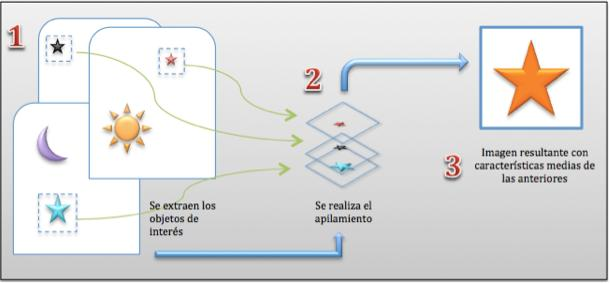
\includegraphics[scale=.5]{image/apilado}
  \end{center}
  \caption{Proceso de apilado de imágenes a partir de un conjunto de
  imágenes normalizadas.}
\end{figure}

\section{Inicios del apilado de imágenes}

Todas las observaciones de imágenes astronómicas poseen un umbral de
sensibilidad por debajo del cual los objetos no son detectables. Si
uno tiene razones para creer que en esa posición del cielo puede
existir algo, basándose en otras observaciones, se puede aplicar
apilamiento a una zona delimitada a un cierto rango de longitudes de
onda, pudiendo variar dicha longitud, y así conseguir el flujo medio
de emisiones.

En una aplicación inicial de esta técnica, Caillault y Helfand,
detectaron el flujo medio de rayos X de estrellas G en Pleiades,
utilizándola para determinar la edad respecto al deterioro de la
emisión. Los detectores de emisiones de rayos X han estado disponible
durante más de dos décadas, por lo que el apilamiento se ha convertido
en una técnica de análisis estándar. Las aplicaciones comenzaron desde
la determinación de la luminosidad media de rayos X, por ejemplo las
galaxias normales, galaxias Lyman y las fuentes de radio, para
determinar la emisión de rayos X de grupos distantes en el
Röntgensatellit (ROSAT) All-Sky Survey.

Los detectores digitales lineales han llegado a dominar los estudios
del cielo óptico e infrarrojo. La técnica de apilamiento ha sido
ampliamente adoptada: por ejemplo, Zibetti et al. detectaron la luz
intracluster apilando Sloan Digital Sky Estudio 683 (SDSS6); Lin et
al., apiló datos sobre las galaxias del cúmulo Two Micron All Sky
Survey (2MASS); Hogg et al. apiló datos del Keck IR para conseguir
galaxias de colores tenues; Minchin et al. fue tan lejos como para
apilar películas digitalizadas desde el telescopio Schmidt del Reino
Unido.
\newpage

\thispagestyle{empty}
\addcontentsline{toc}{section}{Bibliografía}

\nocite{*}
\bibliographystyle{alpha}
\bibliography{report}

\end{document}
